\section{WiFi-Adapter testen}
Vor dem Aufsetzen des Tor-Proxys sollte zuerst überprüft werden, ob der angeschaffte WiFi-Adapter auf dem aufgespielten Betriebssystem lauffähig ist. Dazu steckt man den Adapter in den USB-Port und ruft nach kurzer Wartezeit folgendes Kommando auf:

\begin{lstlisting}
ifconfig -a
\end{lstlisting}

Wenn auf der erschienenen Ausgabe ein Eintrag für \textit{wlan0} zu sehen ist, kann mit der Einrichtung des Access Points begonnen werden.

\begin{figure}[h]
\centering
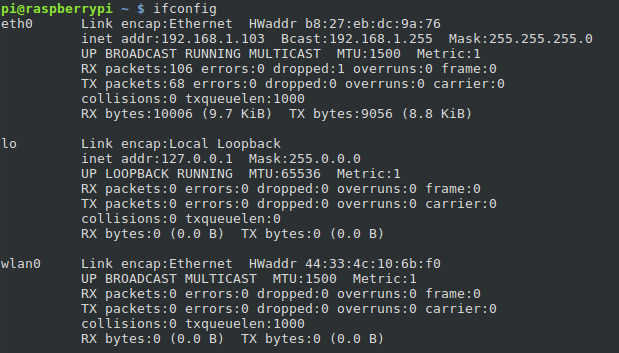
\includegraphics[scale=0.7]{images/ifconfig}
\caption{ifconfig - wlan0}
\end{figure}

\section{Access Point einrichten}
Mit dem eingesteckten Netzwerkkabel und dem per USB angeschlossenen WiFi-Adapter stehen nun zwei Netzwerk-Schnittstellen zur Verfügung. Das Netzwerkkabel hat die Aufgabe, den Raspberry Pi mit dem Internet zu verbinden. Der WiFi-Adapter hingegen soll so eingerichtet werden, dass er ein lokales WLAN aufzieht. Der Raspberry Pi fungiert somit als Wireless Access Point - in deutscher Sprache so viel wie "kabelloser Zugangspunkt". Ein Access Point ermöglicht es Geräten wie Notebooks oder Smartphones, sich über ihn kabellos mit dem Internet zu verbinden. Neben der Software für den Access Point wird ein eigener DHCP-Server benögtigt. Dieser ist dafür verantwortlich, dass jeder Computer, der sich mit dem WLAN verbindet, eine valide IP-Adresse erhält und somit ein Teil des Netzes werden kann.
\\
Mit den folgenden befehlen werden die benötigten Softwarekomponenten installiert.
 
\begin{lstlisting}
apt-get install hostapd isc-dhcp-server
\end{lstlisting}

\subsection{DHCP-Server konfigurieren}
Damit der DHCP-Server auch richtig funktioniert, muss er zuerst konfiguriert werden.
Dazu öffnet man die Datei \textit{/etc/dhcp/dhcpd.conf} mit einem beliebigen Texteditor. In diesem Tutorial wird dazu und für alle nachfolgenden Fälle der vorinstallierte Texteditor Nano verwendet.
\\
Mit dem folgenden Kommando wird die Textdatei mit Nano geöffnet:

\begin{lstlisting}
nano /etc/dhcp/dhcpd.conf
\end{lstlisting}

Zuerst müssen die folgenden Zeilen gefunden und mittels einer vorangestellten Raute (\#) auskommentiert werden. Auskommentieren bedeutet, dass die Zeile ungültig und somit nicht mehr aktiv ist.

\begin{lstlisting}
option domain-name "example.org"
option domain-name-server ns1.example.org,ns2.example.org
\end{lstlisting}

Neu sieht das Ganze folgendermassen aus:

\begin{lstlisting}
#option domain-name "example.org"
#option domain-name-server ns1.example.org,ns2.example.org
\end{lstlisting}

Als Nächstes muss dem DHCP-Server mitgeteilt werden, dass er der offizielle DHCP-Server des zu erstellenden WLAN-Netzes ist. Einmal eingestellt vergibt er fortan valide IP-Adressen an jeden Client, der ihn per DHCP-Request anfragt.
\\
Dazu muss folgende Zeile einkommentiert - die vorangestellte Raute entfernt - werden:

\begin{lstlisting}
#authoritative;
\end{lstlisting}

Die Zeile sollte nun so aussehen:

\begin{lstlisting}
authoritative;
\end{lstlisting}

Das künftig vom WiFi-Adapter aufzuziehende WLAN, für das der DHCP-Server verantwortlich ist, muss einen eigenen Bereich zugewiesen bekommen.
\\
Dazu einfach die folgenden Zeilen ans Ende der Datei anfügen:

\begin{lstlisting}
subnet 192.168.66.0 netmask 255.255.255.0 {
  range 192.168.66.10 192.168.66.50;
  option broadcast-address 192.168.66.255;
  option routers 192.168.66.1;
  default-lease-time 600;
  max-lease-time 7200;
  option domain-name "local";
  option domain-name-servers 8.8.8.8, 8.8.4.4;
}
\end{lstlisting}

Den DHCP-Server ist fertig konfiguriert. Jetzt muss er an ein Netwerkinterface (auf deutsch: Netzwerkschnittstelle) gebunden werden. Das gesuchte Netzwerkinterface ist in diesem Fall wlan0, wie man schon zu beginn mittels ``ifconfig'' herausgefunden hat.
In der Datei \textit{/etc/default/isc-dhcp-server} muss dazu bei der Einstellung \textit{INTERFACES} wlan0 eingetragen werden:

\begin{lstlisting}
INTERFACES="wlan0"
\end{lstlisting}

Dem Interface \textit{wlan0} kann jetzt eine fixe IP-Adresse vergeben werden. Es handelt sich dabei um jene Adresse, die bei der Konfiguration des DHCP-Server bei \textit{option routers} angegeben wurde (192.168.66.1). 
\\
In der Datei \textit{/etc/network/interfaces} müssen folgende Zeilen auskommentiert werden:

\begin{lstlisting}
iface wlan0 inet manual
wpa-roam: /etc/etc/wpa_supplicant/wpa_supplicant.conf
iface default inet dhcp
\end{lstlisting}

Anschliessend fügt man folgende Zeilen hinzu:

\begin{lstlisting}
iface wlan0 inet static
  address 192.168.66.1
  netmask 255.255.255.0
\end{lstlisting}

\begin{figure}[h]
\centering
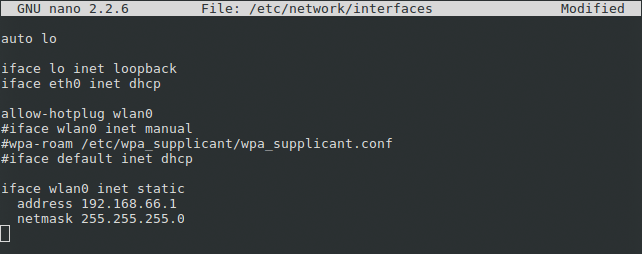
\includegraphics[scale=0.7]{images/network_interfaces}
\caption{konfigurierte interfaces-Datei}
\end{figure}

Das Interface \textit{wlan0} läuft zu diesem Zeitpunkt bereits. Um die eben getätigten Einstellungen sofort wirksam zu machen, muss folgendes Kommando abgesetzt werden:

\begin{lstlisting}
ifconfig wlan0 192.168.66.1
\end{lstlisting}

\subsection{Hostapd konfigurieren}
Jetzt muss der Access Point selbst konfiguriert werden. Die Konfigurationsdatei für \textit{hostapd} existiert aber noch nicht. Deshalb muss man zuerst eine erstellen:

\begin{lstlisting}
touch /etc/hostapd/hostapd.conf
\end{lstlisting}

Die Datei sollte jetzt erstellt sein und kann mit einem Texteditor geöffnet werden:

\begin{lstlisting}
nano /etc/hostapd/hostapd.conf
\end{lstlisting}

Folgende Zeilen muss man hinzufügen:

\begin{lstlisting}
interface=wlan0
driver=rtl871xdrv
ssid=PiProxy
hw_mode=g
channel=6
macaddr_acl=0
auth_algs=1
ignore_broadcast_ssid=0
wpa=2
wpa_passphrase=Test1234
wpa_key_mgmt=WPA-PSK
wpa_pairwise=TKIP
rsn_pairwise=CCMP
\end{lstlisting}

Ein paar der obigen Werte kurz erklärt: 
\begin{itemize}
\item driver: Der Treiber des Wifi-Adapters
\item ssid: Der Name des Netzes, wie man es nach aussen hin sieht
\item wpa\_passphrase: Passwort für den Zugang zum Netz
\end{itemize}

\textit{hostapd} kennt diese Konfiguration noch nicht. Um diese bekanntzumachen, muss in der Datei \textit{/etc/default/hostapd} nach \textit{DAEMON\_CONF} gesucht und die Zeile wie folgt geändert werden:

\begin{lstlisting}
DAEMON_CONF="/etc/hostapd/hostapd.conf"
\end{lstlisting}

Der Raspberry Pi (Tor-Proxy) kann nun auf der einen Seite ein WLAN aufziehen und sich auf der anderen Seite mit dem Internet verbinden. Was jetzt noch fehlt ist die Verbindung dazwischen.

\subsection{NAT konfigurieren}
NAT (Network Address Translation) wird verwendet, um die mit dem WLAN verbundenen Geräte ins Internet weiterzuleiten. Der Datei \textit{/etc/sysctl.conf} muss dazu folgende Zeile angefügt werden:

\begin{lstlisting}
net.ipv4.ip_forward=1
\end{lstlisting}

Folgender Befehl macht die Einstellung aktiv:

\begin{lstlisting}
echo 1 > /proc/sys/net/ipv4/ip_forward
\end{lstlisting}

Zusätzlich muss die Firewall so eingestellt werden, dass NAT die eingerichtete Weiterleitung durchführen kann:

\begin{lstlisting}
iptables -t nat -A POSTROUTING -o eth0 -j MASQUERADE

iptables -A FORWARD -i eth0 -o wlan0 -m state --state RELATED,ESTABLISHED -j ACCEPT

iptables -A FORWARD -i wlan0 -o eth0 -j ACCEPT
\end{lstlisting}

Damit man diese Befehle nicht bei jedem Neustart des Raspberry Pi eingeben muss, können sie permanent gespeichert werden:

\begin{lstlisting}
iptables-save > /etc/iptables.ipv4.nat
echo "up iptables-restore < /etc/iptables.ipv4.nat" >> /etc/network/interfaces
\end{lstlisting}

\section{Aufstarten von hostapd und dem DHCP-Server}
Der Access Point ist jetzt fertig eingerichtet. Um zu überprüfen, ob man alles richtig gemacht hat, muss das Programm zusammen mit der Konfigurationsdatei aufgerufen werden:
\begin{lstlisting}
/usr/sbin/hostapd /etc/hostapd/hostapd.conf
\end{lstlisting}

Entspricht die Ausgabe der unten Abgebildeten, kann das nachfolgende Kapitel übersprungen werden.

\begin{figure}[h]
\centering
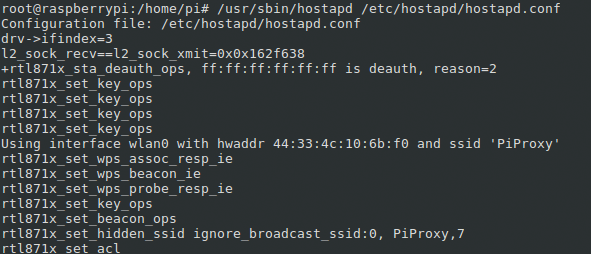
\includegraphics[scale=0.7]{images/hostapd_firststart}
\caption{hostapd- Ausgabe vom Erststart}
\end{figure}

\subsection{Fehlerbehandlung}
Tritt ein Fehler auf, liegt das möglicherweise an einer Inkompatibilität zwischen \textit{hostpad} und dem WiFi-Adapter bzw. dessen Treiber. Bei dem in diesem Tutorial verwendeten WiFi-Adapter kann das Problem gelöst werden, indem man \textit{hostapd} selber kompilliert. Dazu müssen mehrere Schritte befolgt werden.

Zuerst lädt man von der Hersteller-Seite den Linux-Treiber herunter. Dazu geht man auf \url{http://realtek.com} und navigiert zu Downloads > Communications Network ICs > Wireless LAN ICs > WLAN NIC > IEEE 802.11b/g/n Single-Chip > Software. Dort lädt man den Linux-Treiber für den vom  WiFi-Adapter verwendeten Chipsatz herunter (hier: RTL8192CU).
\\
Den heruntergeladenen Treiber (Zip-Datei) kopiert man von einem USB-Stick in das Home-Verzeichnis des Raspberry Pi. Ist der USB-Stick am Pi angeschlossen, müssen dazu folgende Befehle abgesetzt werden:

\begin{lstlisting}
mount /dev/sda1 /mnt
cp /mnt/RTL8188C_8192C_USB_linux_v4.0.2_9000.20130911.zip /home/pi
\end{lstlisting} 

Jetzt muss die Zip-Datei entpackt werden:

\begin{lstlisting}
cd /home/pi
unzip RTL8188C_8192C_USB_linux_v4.0.2_9000.20130911.zip
\end{lstlisting}

Danach muss ins richtige Verzeichnis gewechselt und das Archiv von für hostapd entpackt werden:

\begin{lstlisting}
cd wpa_supplicant_hostapd
tar -xzvf wpa_supplicant_hostapd-0.8_rtw_r7475.20130812.tar.gz
\end{lstlisting}

Danach muss erneut in das richtige Verzeichnis gewechselt werden:

\begin{lstlisting}
cd wpa_supplicant_hostapd-0.8_rtw_r7475.20130812
cd hostapd
\end{lstlisting}

Im richtigen Verzeichnis angelangt kann hostapd kompiliert werden. Den Kompiliervorgang starten man mit folgendem Befehl:

\begin{lstlisting}
make
\end{lstlisting}

Nach ein paar Minuten Wartezeit steht die frisch kompilierte, binäre Datei bereit. Bevor diese kopiert wird, sollte die Original-Datei gesichert werden:

\begin{lstlisting}
mv /usr/sbin/hostapd /usr/sbin/hostapd.ORIG
\end{lstlisting}

Danach kann die neue \textit{hostapd}-Binärdatei kopiert werden:

\begin{lstlisting}
cp hostapd /usr/sbin	
\end{lstlisting}

Die Dateinamen und Verzeichnisse können sich je nach Fall von den hier Verwendeten unterscheiden und müssen dementsprechend angepasst werden.

\subsection{Access Point testen}
Bevor der Access Point richtig getestet werden kann, müssen alle beteiligten Komponenten gestartet werden:

\begin{lstlisting}
service hostapd start
service isc-dhcp-server start
\end{lstlisting}

Das WLAN ist jetzt aktiv und für jedes WiFi-fähige Geräte erkennbar.

\begin{figure}[h]
\centering
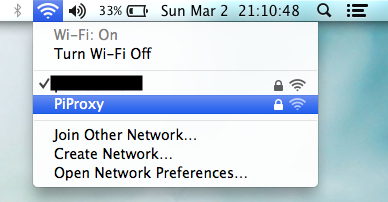
\includegraphics[scale=0.7]{images/accesspoint}
\caption{Der erstellte Access Point}
\end{figure}

Verhält sich der Access Point nicht wie gewünscht oder läuft gar nicht erst, empfiehlt es sich, alle vorherigen Schritte noch einmal zu studieren und die Konfigurationen zu überprüfen. Für schwer zu lösende Probleme kann man sich auch immer an die Internet-Gemeinschaft wenden.

\section{Daemons einrichten}
Beide Komponenten - hostapd und isc-dhcp-server - können als sogenannter "Daemon" eingerichtet werden. Daemons sind Programme, die beim Start des Computers automatisch aufstarten. Man will den Access Point schliesslich nicht jedes Mal manuell über die Konsole starten müssen. 

\begin{lstlisting}
update-rc.d hostapd enable 
update-rc.d isc-dhcp-server enable
\end{lstlisting}

Um die Daemons auf korrekte Funktionsweise zu überprüfen, muss man den PC neu starten:

\begin{lstlisting}
shutdown -r now 
\end{lstlisting}

Ist der PC wieder hochgefahren, fragt man die Stati der beiden Daemons ab:

\begin{lstlisting}
service hostapd status
service isc-dhcp-server status
\end{lstlisting}

Die Ausgabe sollte wie folgt aussehen: 

\begin{figure}[h]
\centering
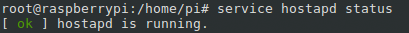
\includegraphics[scale=0.7]{images/hostapd_status}
\caption{Status Access Point}
\end{figure}

\begin{figure}[h]
\centering
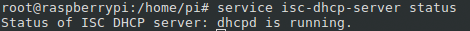
\includegraphics[scale=0.7]{images/dhcp_status}
\caption{Status DHCP-Server}
\end{figure}

\section{Tor aufsetzen}
An dieser Stelle ist es möglich, sich mittels Access Point mit dem Internet zu verbinden. Das Ziel ist es, die Verbindung ins Internet über das Tor-Netzwerk zu leiten. Tor kann man, wie die zuvor verwendeten Programme auch, über die Paketverwaltung installieren:

\begin{lstlisting}
apt-get install tor
\end{lstlisting}

Nach der Installation muss Tor natürlich noch richtig konfiguriert werden: 

\begin{lstlisting}
nano /etc/tor/torrc
\end{lstlisting} 

Direkt nach dem einleitenden Kommentarblock müssen folgende Zeilen hinzugefügt werden:

\begin{lstlisting}
Log notice file /var/log/tor/notices.log
VirtualAddrNetwork 10.192.0.0/10
AutomapHostsSuffixes .onion,.exit
AutomapHostsOnResolve 1
TransPort 9040
TransListenAddress 192.168.66.1
DNSPort 53
DNSListenAddress 192.168.66.1
\end{lstlisting}

Die Datei sollte nun folgendermassen aussehen: 

\begin{figure}[h]
\centering
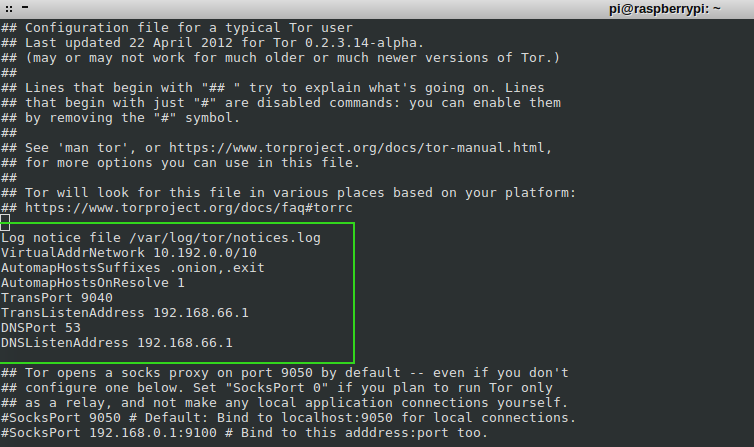
\includegraphics[scale=0.6]{images/torrc}
\caption{torrc-Datei}
\end{figure}
 	
Der Firewall muss jetzt noch beigebracht werden, dass jegliche Kommunikation vom WLAN-Netz über das Tor-Netzwerk weitergeleitet werden soll:

\begin{lstlisting}
iptables -F

iptables -t nat -F

iptables -t nat -A PREROUTING -i wlan0 -p tcp --dport 22 -j REDIRECT --to-ports 22

iptables -t nat -A PREROUTING -i wlan0 -p udp --dport 53 -j REDIRECT --to-ports 53

iptables -t nat -A PREROUTING -i wlan0 -p tcp --syn -j REDIRECT --to-ports 9040

iptables-save > /etc/iptables.ipv4.nat
\end{lstlisting}

In der \textit{torrc}-Konfigurationsdatei wurde bei \textit{Log notice file} eine Datei angegeben, die in Zukunft alle Logs enthält. Diese Datei muss nun erstellt und mit den entsprechenden Rechten versehen werden:

\begin{lstlisting}
touch /var/log/tor/notices.log
chown debian-tor /var/log/tor/notices.log
chmod 644 /var/log/tor/notices.log
\end{lstlisting}

Nun muss man den Tor-Service noch neu starten, damit die vorgenommenen Einstellungen aktiv werden:

\begin{lstlisting}
service tor restart
\end{lstlisting}

Um zu prüfen, ob Tor erfolgreich gestartet werden konnte, kann man folgenden Befehl ausführen:

\begin{lstlisting}
service tor status
\end{lstlisting}

Die Ausgabe sollte ähnlich dieser sein:

\begin{figure}[h]
\centering
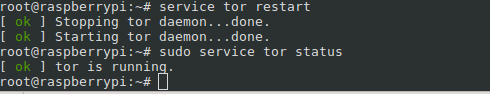
\includegraphics[scale=0.7]{images/tor_service}
\caption{Tor - Neustart und Status}
\end{figure}

Auch Tor soll bei jedem Neustart des Systems automatisch laufen. Um Tor als Daemon zu konfigurieren, muss man analog zu vorhin folgenden Befehl absetzen:

\begin{lstlisting}
update-rc.d tor enable
\end{lstlisting}

Der Access Point und Tor sind an diesem Punkt fertig installiert und eingerichtet. Jetzt fehlt nur noch ein abschliessender Test, um sicherzustellen, dass alles so funktioniert, wie es soll.

\section{IP-Adresse verifizieren}
Mittels \url{http://wieistmeineip.ch} kann die IP-Adresse ermittelt werden, mit der man sich im Internet bewegt. Diese wird einem normalerweise vom Provider zugeteilt und ändert sich eher selten. Mit einem funktionierenden Tor-Setup ändert sich dieses Verhalten jedoch. Da je Anfrage ins Internet drei verschiedene Tor-Server passiert, ändert sich die Absender-IP-Adresse des Paketes jedes Mal. Die angefragte Internetseite sieht somit nie die IP-Adresse, die einem vom Provider zugeteilt wurde, sondern immer die des zuletzt passierten Tor-Servers - auch Exit-Node genannt. Um die korrekte Funktionsweise des Tor-Proxys zu verifizieren, muss man lediglich von einem Computer im normalen Netz und einem Gerät, das mittels Tor-Proxy mit dem Internet verbunden is, die Seite \textit{wieistmeineip} aufrufen. Die IP-Adressen und auch die sonstigen angezeigten Informationen dürfen sich bei einem funktionierende Tor-Proxy nicht decken.


\section{Exit-Nodes konfigurieren}
Der letzte Tor-Server auf dem Weg zum Ziel ist der Exit-Node. Er hat die Aufgabe, das Paket an das Ziel weiterzuleiten. Dazu muss er aber zuerst das Paket aus den verschiedenen Schichten auspacken - es entschlüsseln - um die Zieladresse zu lesen. Dadurch kann er unter Umständen den Inhalt des Pakets ermitteln und es mit der Empfängerinformation in einen grösseren Zusammenhang stellen. Da jeder einen solchen Exit-Node betreiben kann - gut gesinnte Privatpersonen oder Organisationen, Geheimdienste oder sonstige Kriminelle - kann man nie genau wissen, wer jetzt einen sogenannten "Bad-Exit-Node" betreibt. Glücklicherweise kann das Risiko minimiert werden. In der Tor-Konfigurationsdatei \textit{torrc} kann man festlegen, welche Exit-Nodes verwendet werden sollen. Es gibt diverse Organisationen und Verbünde, die solche Tor-Exit-Nodes betreiben und zum Gebrauch anbieten. Eine davon ist die Swiss Privacy Foundation: \url{http://privacyfoundation.ch/}.
\\
Um die Exit-Nodes einzuschränken bzw. nach seinen persönlichen Wünschen zu selektieren, gibts es zwei Möglichkeiten, die sich mitunter sogar kombinieren lassen: 

\begin{enumerate}
\item Angabe des "Fingerprints" (eindeutige ID) eines spezifischen Exit-Nodes
\item Angabe eines Ländercodes, wodurch nur Exit-Nodes von diesem Land verwendet werden
\end{enumerate}

Die Einstellungen werden in der \textit{torrc}-Konfigurationsdatei vorgenommen. Diese  muss man zuerst mittels Texteditor öffnen:

\begin{lstlisting}
nano /etc/tor/torrc
\end{lstlisting}

Die folgenden Zeilen werden nach \textit{DNSListenAddress 192.168.66.1} angefügt:

\begin{lstlisting}
StrictNodes 1
ExitNodes Fingerprint,{Laendercode},...
\end{lstlisting}

"Fingerprint" ist eine lange Kombination aus Zahlen und Buchstaben mit einem vorangestellten \$-Zeichen. Beispielsweise hat ein von der Swiss Privacy Foundation bereitgestellter Exit-Node den Fingerprint \$944224E9413705EEAFCBAC98BF57C475EB1960C5.
Zwischen den geschweiften Klammern kann ein Ländercode angegeben werden. Für Exit-Nodes aus der Schweiz müsste man \{ch\} verwenden. Man kann dabei so viele Länder angeben wie man will. 
\\
Wichtig ist, dass alle angegebenen Optionen (Ländercodes und Fingerprints) stets mittels Komma getrennt werden und keine Leerzeichen dazwischenstehen.
\\
Ein weiteres Beispiel soll ein bisschen Klarheit schaffen:

\begin{lstlisting}
ExitNodes $944224E9413705EEAFCBAC98BF57C475EB1960C5,{de},{at}
\end{lstlisting}

Mit dieser Einstellung werden nur deutsche und österreichische Exit-Nodes verwendet inklusive einem zu Bginn einzeln definierten Exit-Node.

\section{Abschluss}
Tor bietet noch viele andere Möglichkeiten, den Dienst den eigenen Ansprüchen anzupassen und sicherer zu machen. Details zu den unterschiedlichen Konfigurationen und Modi findet man hier: \url{https://www.torproject.org/docs/tor-manual.html.en}. Die Seite ist zur Zeit leider nur auf Englisch verfügbar. Sicherlich findet man auch im Internet allerhand Material, um die eigenen Bedürfnisse zu decken.